%%%%%%%%%%%%%%%%%%%%%%%%%%%%%%%%%%%%%%%%%%%%%%%%%%%%%%%%%%%%%%%%%%%%%%%%%%%
%
%    phase1-AR.tex  (use only for Archival Research and Theory proposals; use phase1-GO.tex
%                     for General Observer and Snapshot proposals and phase1-DD.tex for GO/DD 
%                     proposals or use phase1-MC.tex for GO/MC rapid response proposals.
%                     
%
%    HUBBLE SPACE TELESCOPE
%    PHASE I ARCHIVAL & THEORETICAL RESEARCH PROPOSAL TEMPLATE 
%    FOR CYCLE 24 (2016)
%
%    Version 1.1, August 12,  2015.
%
%    Guidelines and assistance
%    =========================
%     Cycle 23 Announcement Web Page:
%
%         http://www.stsci.edu/hst/proposing/docs/cycle23announce 
%
%    Please contact the STScI Help Desk if you need assistance with any
%    aspect of proposing for and using HST. Either send e-mail to
%    help@stsci.edu, or call 1-800-544-8125; from outside the United
%    States, call [1] 410-338-1082.
%
%%%%%%%%%%%%%%%%%%%%%%%%%%%%%%%%%%%%%%%%%%%%%%%%%%%%%%%%%%%%%%%%%%%%%%%%%%%

% The template begins here. Please do not modify the font size from 12 point.

\documentclass[12pt]{article}
\usepackage{phase1}

\usepackage{graphicx}
%\usepackage{amssymb}

\usepackage{wrapfig}
\usepackage{setspace}
%\usepackage{subfigure}
\usepackage{subcaption}
\usepackage{mathtools}



\graphicspath{/Users/David/Research_Documents/inclination/git_inclination/pilot_paper_code/pilot_paper/paper_figures2/}

\begin{document}

%   1. SCIENTIFIC JUSTIFICATION
%       (see Section 9.1 of the Call for Proposals)
%
%
\justification          % Do not delete this command.
% Enter your scientific justification here.

%The majority of the baryons in the universe are found in the intergalactic medium (IGM). The properties of this important reservoir of matter are most directly measured via absorption in the spectra of UV-bright background QSOs. The UV initiatives undertaken by the Cosmic Origins Spectrograph on HST have produced a wealth of high resolution and high signal-to-noise spectra that are ideal for a wide variety of IGM studies. However, the identification and measurement of spectral features is a major undertaking, and limits the viability of large-scale studies using archival HST data. We propose to create a legacy data archive of all archival COS sightlines, complete with line identifications and measurements. In addition, we will match nearby ($cz \leq 10,000$ km/s) spectral features with probable associated galaxies using the likelihood method we have developed (French et al. 2016, in prep). This will be the first large, publicly accessible IGM absorber dataset, and will provide a legacy artifact directly in line with the NASA Mission Directive whatever-it's-call-thing.

\indent \indent The majority of the baryons in the universe are found in the intergalactic and circumgalactic medium (IGM, CGM) (e.g. Danforth $\&$ Shull 2008, Lehner et al. 2007, Cen 2013 and references therein). Galaxies reside within large filaments of IGM gas, and draw new material from it for continuing star formation, as well as eject enriched material back into it. Studying this complex process observationally is challenging, yet paramount to properly understanding and modeling global galaxy evolution.

The properties of this reservoir of matter are most directly measured via absorption in the spectra of UV-bright background QSOs. Studies using this method have found numerous IGM-galaxy proximity effects, such as absorption equivalent width (CITE), linewidth (e.g. Wakker $\&$ Savage 2009), column density (e.g. Rudie et al 2012), and metallicity (e.g. Kacprzak et al YEAR?) decreasing with the distance to the nearest bright galaxy. 

Nevertheless, many open questions remain concerning the details of how gas near to galaxies (the CGM, generally considered to extend to $\sim 2R_{vir}$) interacts with and affects the evolution of the galaxies. Some key questions we would like to answer are:
a) how do the properties of CGM absorbers (e.g. equivalent width, location, velocity) compare to the properties of the galaxies they are associated with (e.g. size, inclination, morphology)?
b) does the CGM follow the rotation direction and velocity of the associated galaxies as predicted by simulations (e.g. Stewart et al. 2011)?

%Additionally, by limiting the redshift of our sample, we can include large angular and physical impact parameters, which allows for a wider search for associated QSO sightlines.

Probing gas both very near to as well as physically far from a galaxy is essential to developing a full understanding of the galaxy-IGM interface. This is most easily done in the nearby universe, where the galaxy sample is highly complete to low luminosities. However, previous studies have suffered from several shortcomings in trying to address these questions. We propose a program to deal with the following 3 issues in particular:\\

\noindent 1) \textbf{\underline{Incompleteness}}: As the completeness of known galaxies decreases sharply with redshift, many CGM studies suffer form limitations due to inhomogeneity and incompleteness in the galaxy data. For example, Mathes et al. (2014) and Werk et al. (2014) are only complete to $\sim L^{\**}$ (at $0.12 < z < 0.67$ and $z\sim0.2$, respectively). This complicates the process of associating absorption with a nearby galaxy, and can result in significant biases. Additionally, very few galaxies have published rotation curves, so comparing the velocity of the gas in the CGM to that within the disks of the associated galaxies is usually not possible. Aside from general incompleteness, distant galaxies also tend to have less detailed information (e.g. inclination, position angle, size), and are more prone to misclassification.

To correct for this, we are limiting our study to the redshift range $400$ $\leq$ $cz$ $\leq$ $10,000$ km/s, where available galaxy data is complete to $\sim0.2 L^{\**}$ at $10,000$ km/s, and progressively better towards lower redshifts. We have created a nearby galaxy catalog to aid in our analysis by mining the NASA Extragalactic Database (NED), collecting redshifts, diameters, redshift-independent-distances, morphologies, inclinations, position angles, photometry, and more for each galaxy, and then normalizing these values beyond the basic work done by NED. This catalog is the most complete, comprehensive and up-to-date nearby galaxy catalog in existence (to be published in 2016), and is key to allowing us to draw direct comparisons between the properties of the absorbers in the CGM and the properties of galaxies on a larger scale then ever before.

We have also secured Priority 1 time on the Southern African Large Telescope (SALT) to measure the rotation curves of 15+ galaxies with sightlines lying within $2R_{vir}$. With this data in hand we will compare the rotation and orientation of the galaxies with that of Ly$\alpha$ absorption detected in their halos. \\



\noindent 2) \textbf{\underline{Reproducibility}}: In order to correlate CGM absorber properties with a galaxy, a match must be made between a galaxy to an absorption feature, but it is often unclear or arbitrary how this matching is done. Some (e.g. CITATION) simply picked the closest neighboring galaxy to the detected IGM absorber, while others (e.g. CITATION) try to take galaxy size and other properties into account as well. However, different authors continue to use different, subjective criteria, and tend to deal with ambiguities in an ad-hoc manner.

\textbf{Likelihood Method:} In French et al. (2016, in prep) we are introducing a reproducible, likelihood-based method to streamline these types of decisions. We define the likelihood as follows:

\begin{equation}
	\mathcal{L} = e^{-(\rho/R_{vir})^2} e^{-(\Delta v / 200)^2},
\end{equation}
where $\rho$ is the physical impact parameter between the sightline and a galaxy, $R_{vir}$ is the galaxy's virial radius, and $\Delta v = v_{galaxy} - v_{absorber}$, the difference in velocity between the galaxy and the absorption line. In order for a galaxy to be deemed ``associated" with an absorption line, we require $\mathcal{L}$ for any potentially associated galaxy be a factor of 5 larger than $\mathcal{L}$ for all other galaxies, and $\mathcal{L} \geq 0.001$. This hard limit translates to an absorber located at $\sim 2 R_{vir}$ and $\sim 350$ km/s in physical and velocity separation, respectively. This edge agrees nicely with observational results of \textbf{EXAMPLES AND REFERENCES}.\\


\begin{figure}[t!]
    \centering
    \begin{subfigure}[t]{0.5\textwidth}
        \centering
        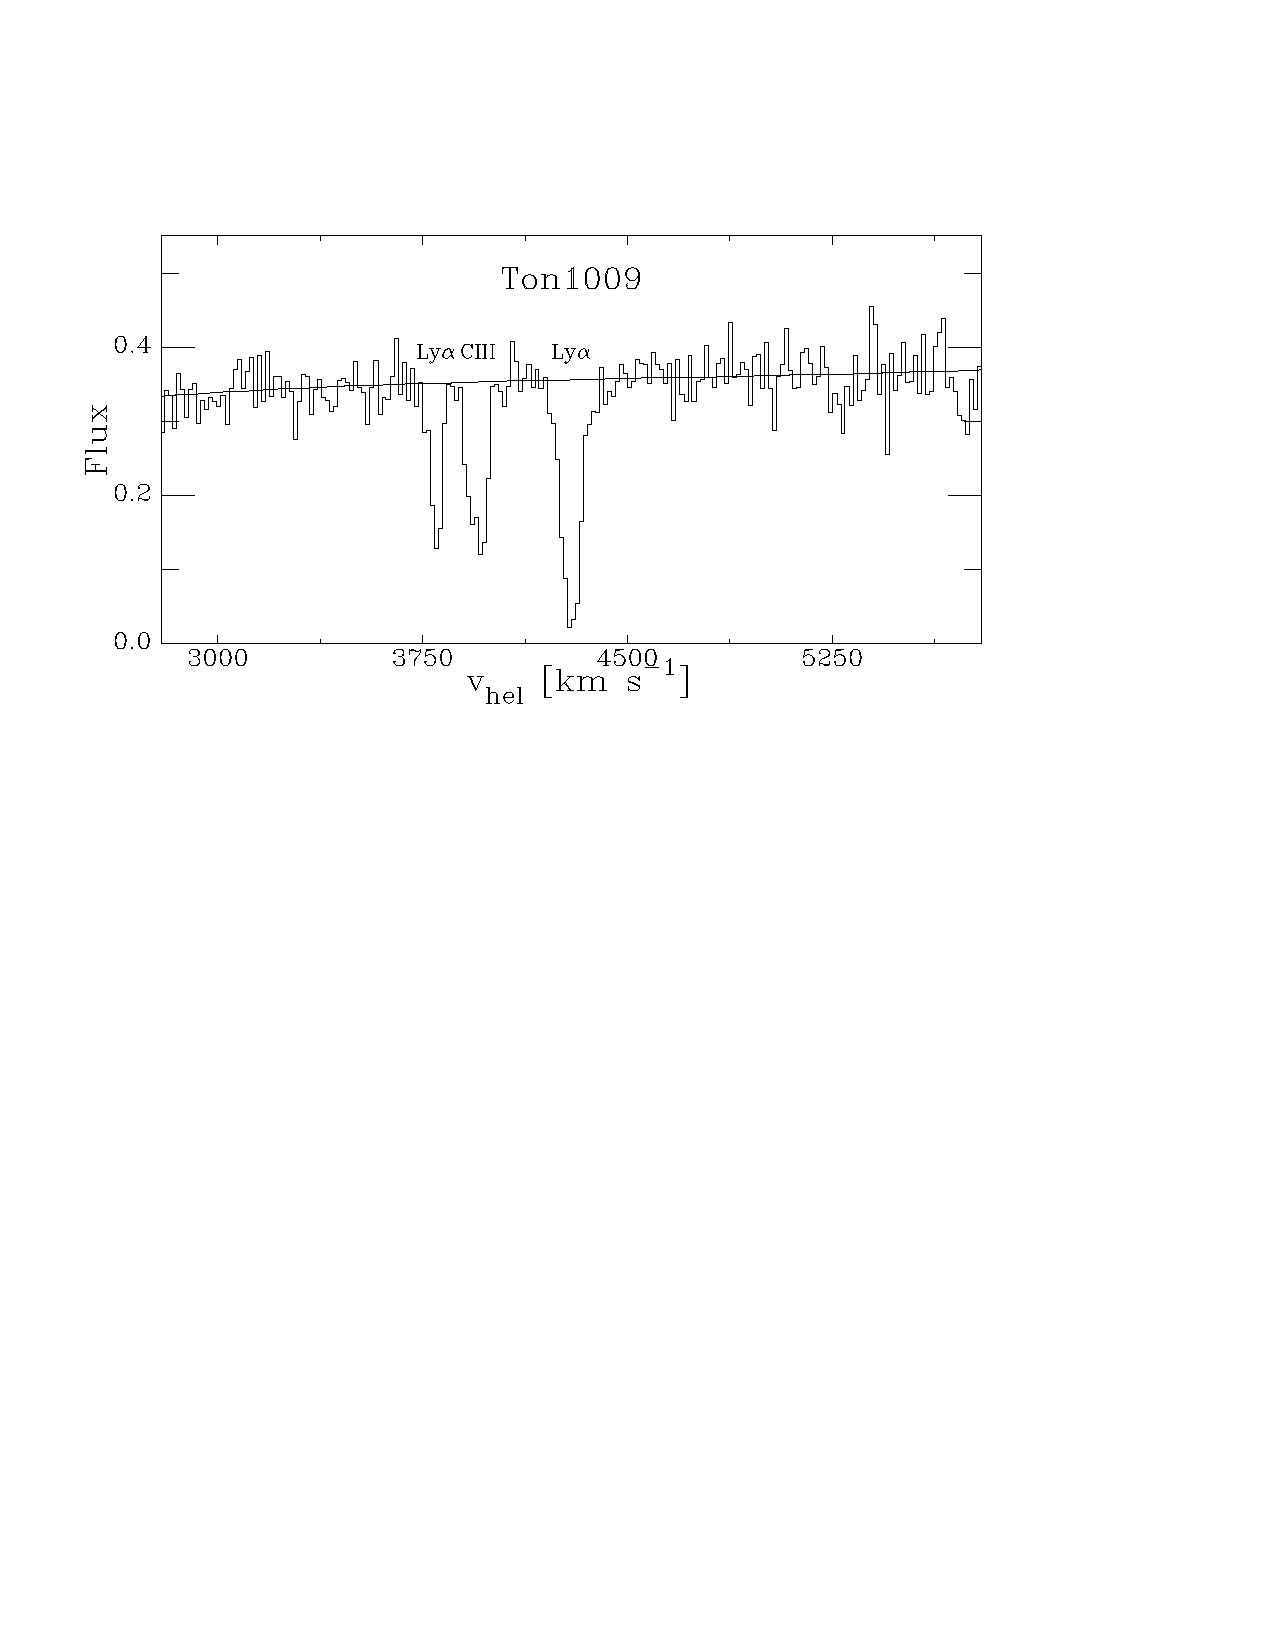
\includegraphics[width=\textwidth]{figTON1009_crop.pdf}
        \caption{}
    \end{subfigure}%
    ~ 
    \begin{subfigure}[t]{0.5\textwidth}
        \centering
        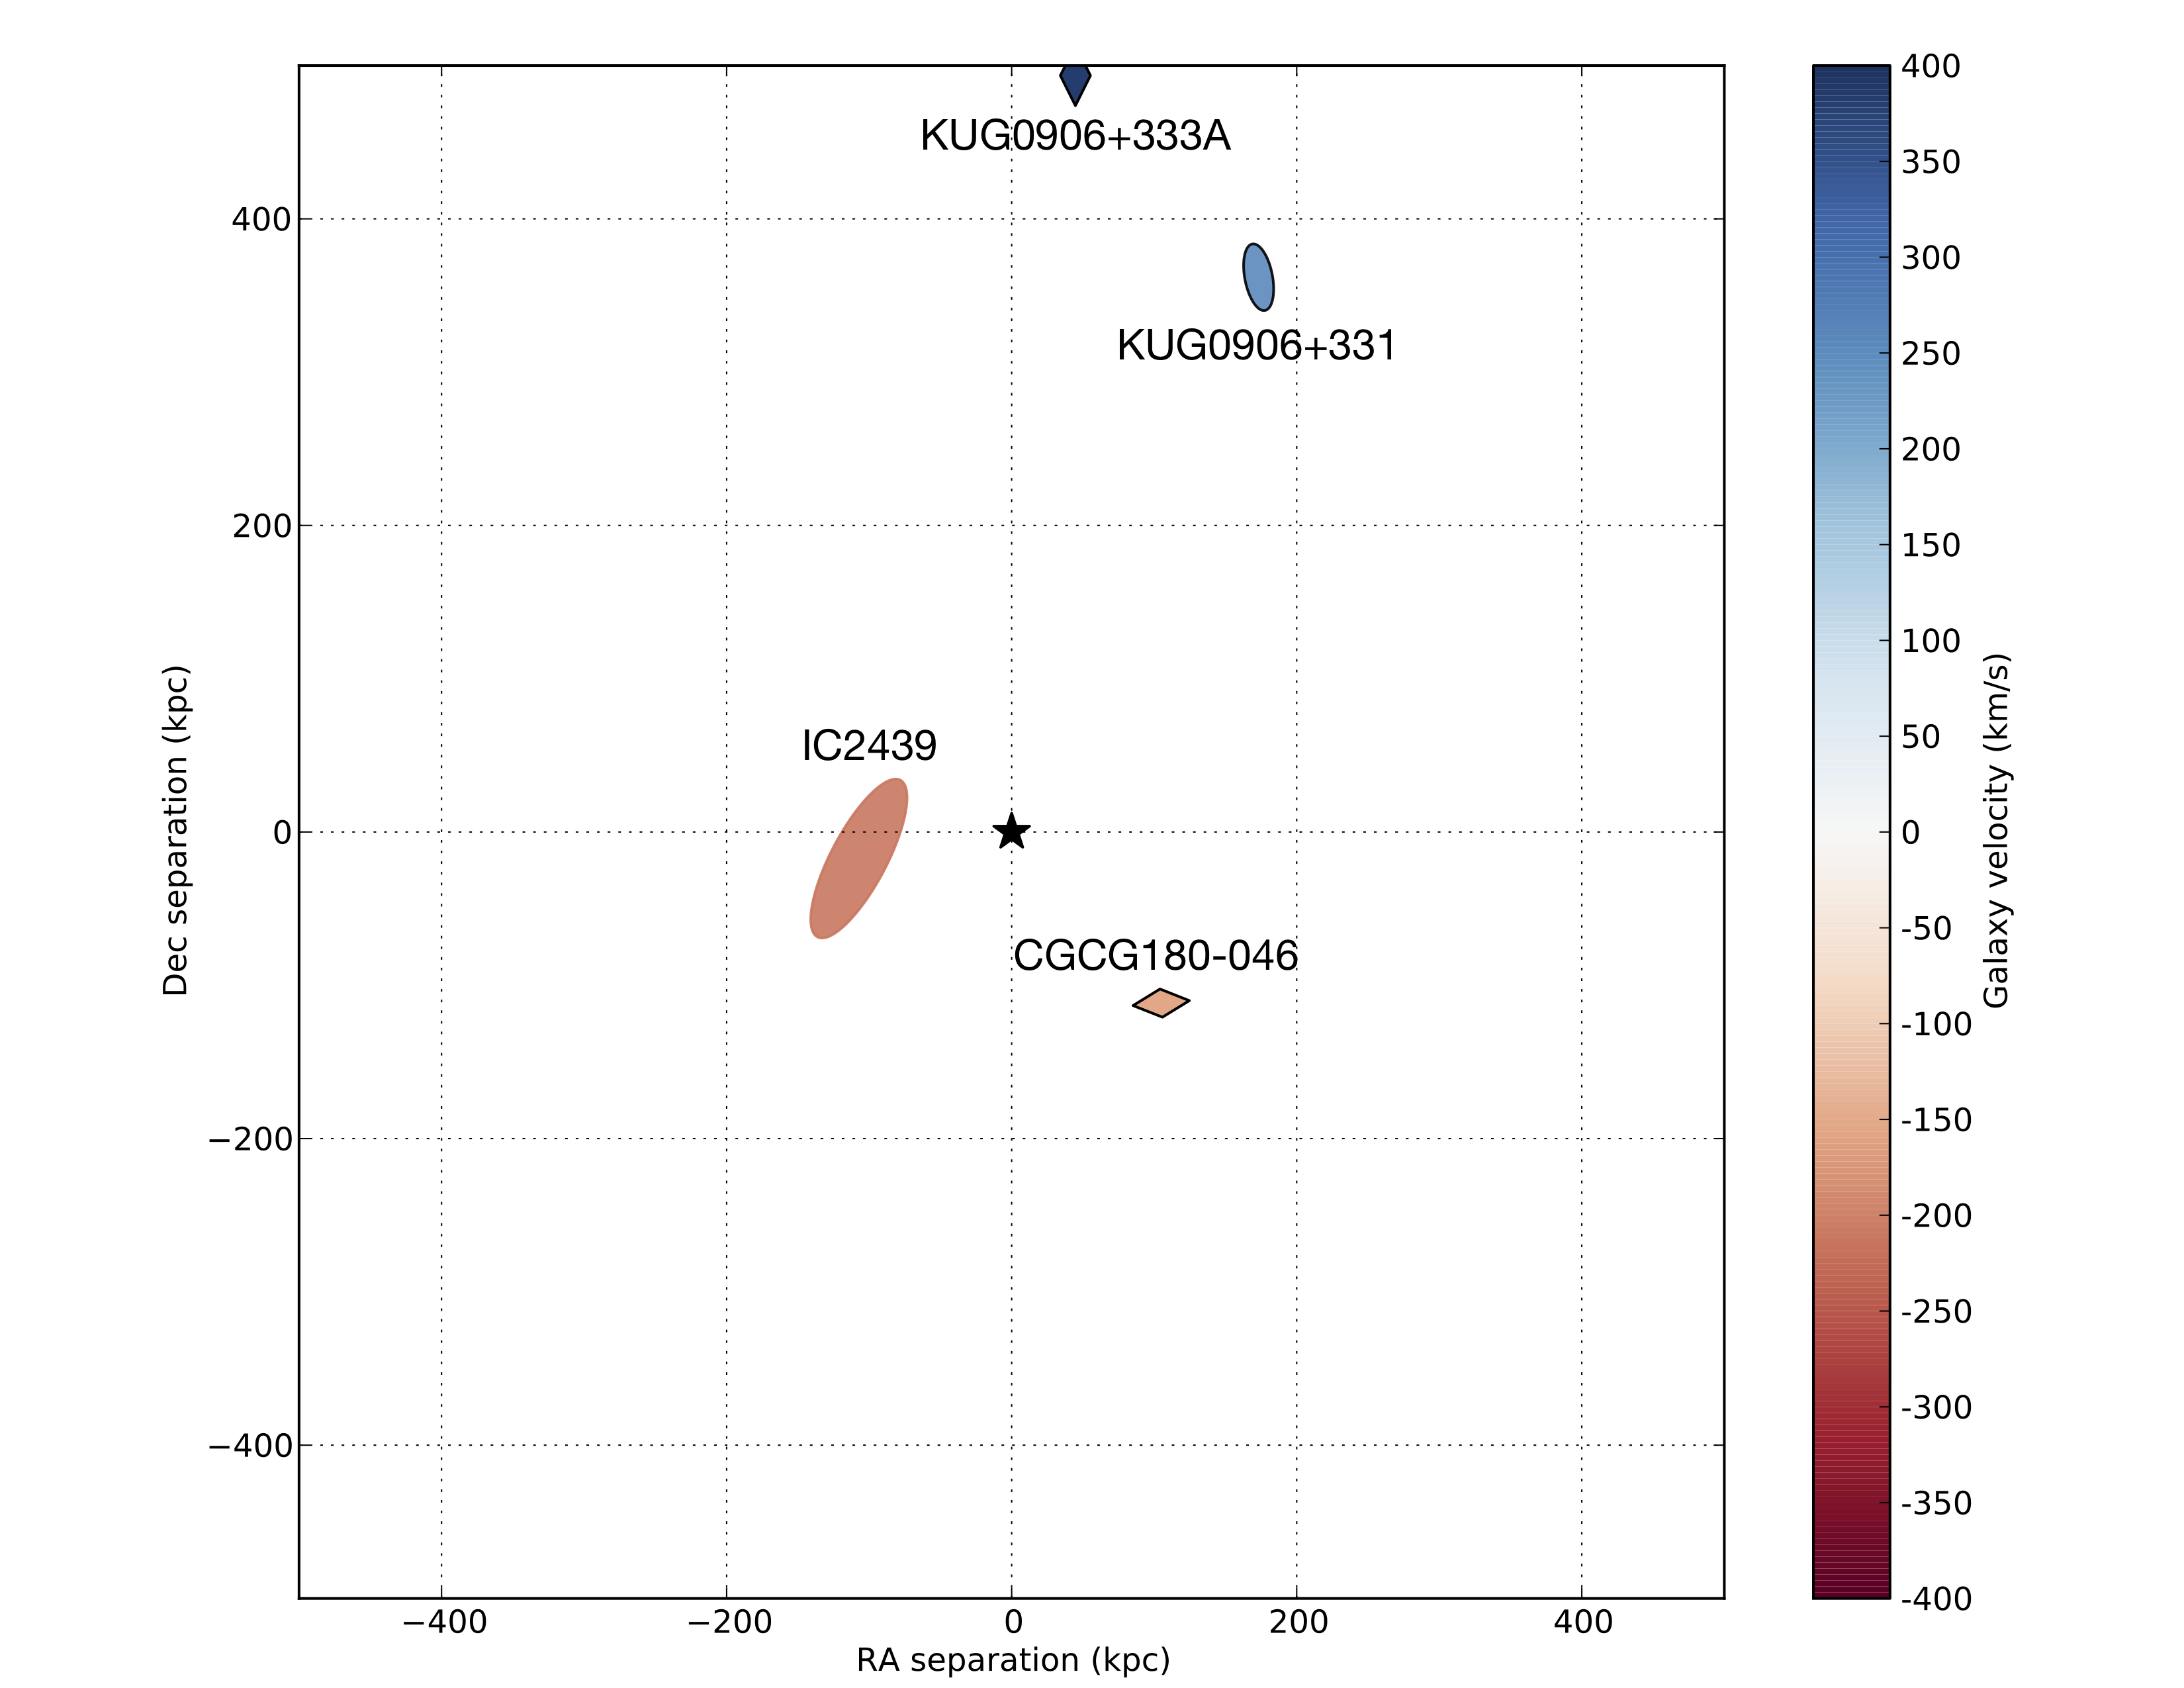
\includegraphics[width=\textwidth]{map_TON1009_4285_crop2_labels.png}
        \caption{}
    \end{subfigure}
  \caption{\small{a) An example Ly$\alpha$ line found in a sightline towards target TON1009 at 4295 km/s. b) A map of \textit{all} galaxies within a 500 kpc impact parameter target TON1009 sightline and with velocity ($cz$) within 400 km/s of absorption detected at 4295 km/s (central black star). The galaxy IC2439 ($v=4494$ km/s, inclination = $71^{\circ}$) can be unambiguously paired with the Ly$\alpha$ absorption feature at $v=4295$ km/s following our selection criteria ($\mathcal{L}_{IC2439} = 0.45$, many times larger than all other nearby galaxies).}}
  \vspace{-10pt}
%    \caption{Caption place holder}
\end{figure}



\noindent 3) \textbf{\underline{Sample size}}: Probing the CGM in absorption requires a serendipitously located background source, which means that a particular galaxy halo generally only can be probed once. It is thus necessary to study the statistics of a large dataset of single galaxy-absorber matches. However, the largest current CGM surveys max out at fewer than 100 galaxy-absorber pairs (e.g. 93 in Wakker $\&$ Savage 2009, 44 in Tumlinson et al. 2013, 89 in Steidel et al 2010, 71 in Stocke et al 2013).

\textbf{Archival data:} At the time of writing 550 QSO targets have been observed with COS. 300 spectra have S/N$\geq$10; of these 120 have $0.03\leq z \leq 0.2$, such that intrinsic Ly$\alpha$ is in the G130M wavelength range, 90 have $0.2\leq z \leq 0.45$, putting Ly$\alpha$ in G160M, and 90 have $z > 0.45$. Nearly all of these pass within 500 physical kpc of at least one galaxy in the $cz \leq 10,000$ km/s redshift range. In our pilot study of 35 sightlines (French et al. 2016, in prep), we measured 176 Ly$\alpha$ absorption lines, 42 of which we paired with nearby galaxy using our likelihood method. Hence, we predict 300 total spectra should produce over 1500 absorption lines and 360 absorber-galaxy pairings.

\textbf{Line Identification}: The identification and measurement of spectral features is a major undertaking, and limits the viability of large-scale studies using archival HST data. To combat this we have developed a pipeline that helps automate the IDing of targets, which will allow us to produce a sample of hundreds of spectra and thousands of absorption lines. As the final step of our proposed program, we will create a legacy data archive of identifications and measurements of COS sightlines, complete with probable galaxy associations.\\


\noindent \underline{\textbf{4. Summary}}

Galaxies have a complex relationship with their environment, and are known to both eject and accrete material from the surrounding IGM. Although many studies have probed this CGM gas, none yet have overcome the issues of incompleteness, small sample size, and reproducibility. We propose a large scale survey to overcome these common shortcomings, and provide robust statistics on how the properties of Ly$\alpha$ absorption depend on the properties of nearby galaxies. We will select 300 of the 550 available COS sightlines to ID and cross-correlate with our nearby galaxy catalog, and produce the largest yet galaxy-absorber catalog. This will also provide a legacy dataset of ID'd and measured absorption lines for a majority of COS sightlines, which will continue to be useful to the community long after the end of this project.

%We propose to complete a large scale program to address these issues by using archival COS sightlines to target nearby galaxy-absorber systems. The following sections will discuss in detail how our proposed program address each of the above issues.\\

%and $z \geq 0.03$, the minimum to be useful for our purposes (anything $z \leq 0.03$, or $cz \leq 10,000$ km/s, is too close to the galaxy velocities). These break down into 3 redshift bins, with 120 at $0.03\leq z \leq 0.2$, 90 at $0.2\leq z \leq 0.45$ and another 90 at $z > 0.45$. 

%In attempt to combat these issues, we have begun a large scale survey of nearby COS sightline-galaxy associations, restricting ourselves to $cz \leq 10,000$ km/s, where we have assembled a galaxy catalog complete to $L^{\**}\sim 0.1$. To address the reproducibility issue, we have developed a probability algorithm to automatically choose which galaxy to associate an absorption line with. 
%
%Finally, we have been awarded priority 1 time on the Southern Africa Large Telescope (SALT) in order to measure the rotation curves of 15+ galaxies that have absorption detected in a sightline within 300 kpc and 400 km/s of the galaxy. This data combined with archival COS sightlines will allow us to finally probe how the kinematics of the CGM compare to that of the gas within the disks of galaxies.



%Studies of the circumgalactic medium, or the IGM-galaxy connection, generally rely on matching absorption measured in the spectra of background QSOs to a nearby foreground galaxy. The methods used for matching a galaxy to an IGM absorber are universally ad-hoc, however, and range from picking the nearest galaxy in physical impact parameter, to some combination of impact parameter, size, and judgement. 


%\begin{figure}[ht!]
%\centering
%  \subfigure[]{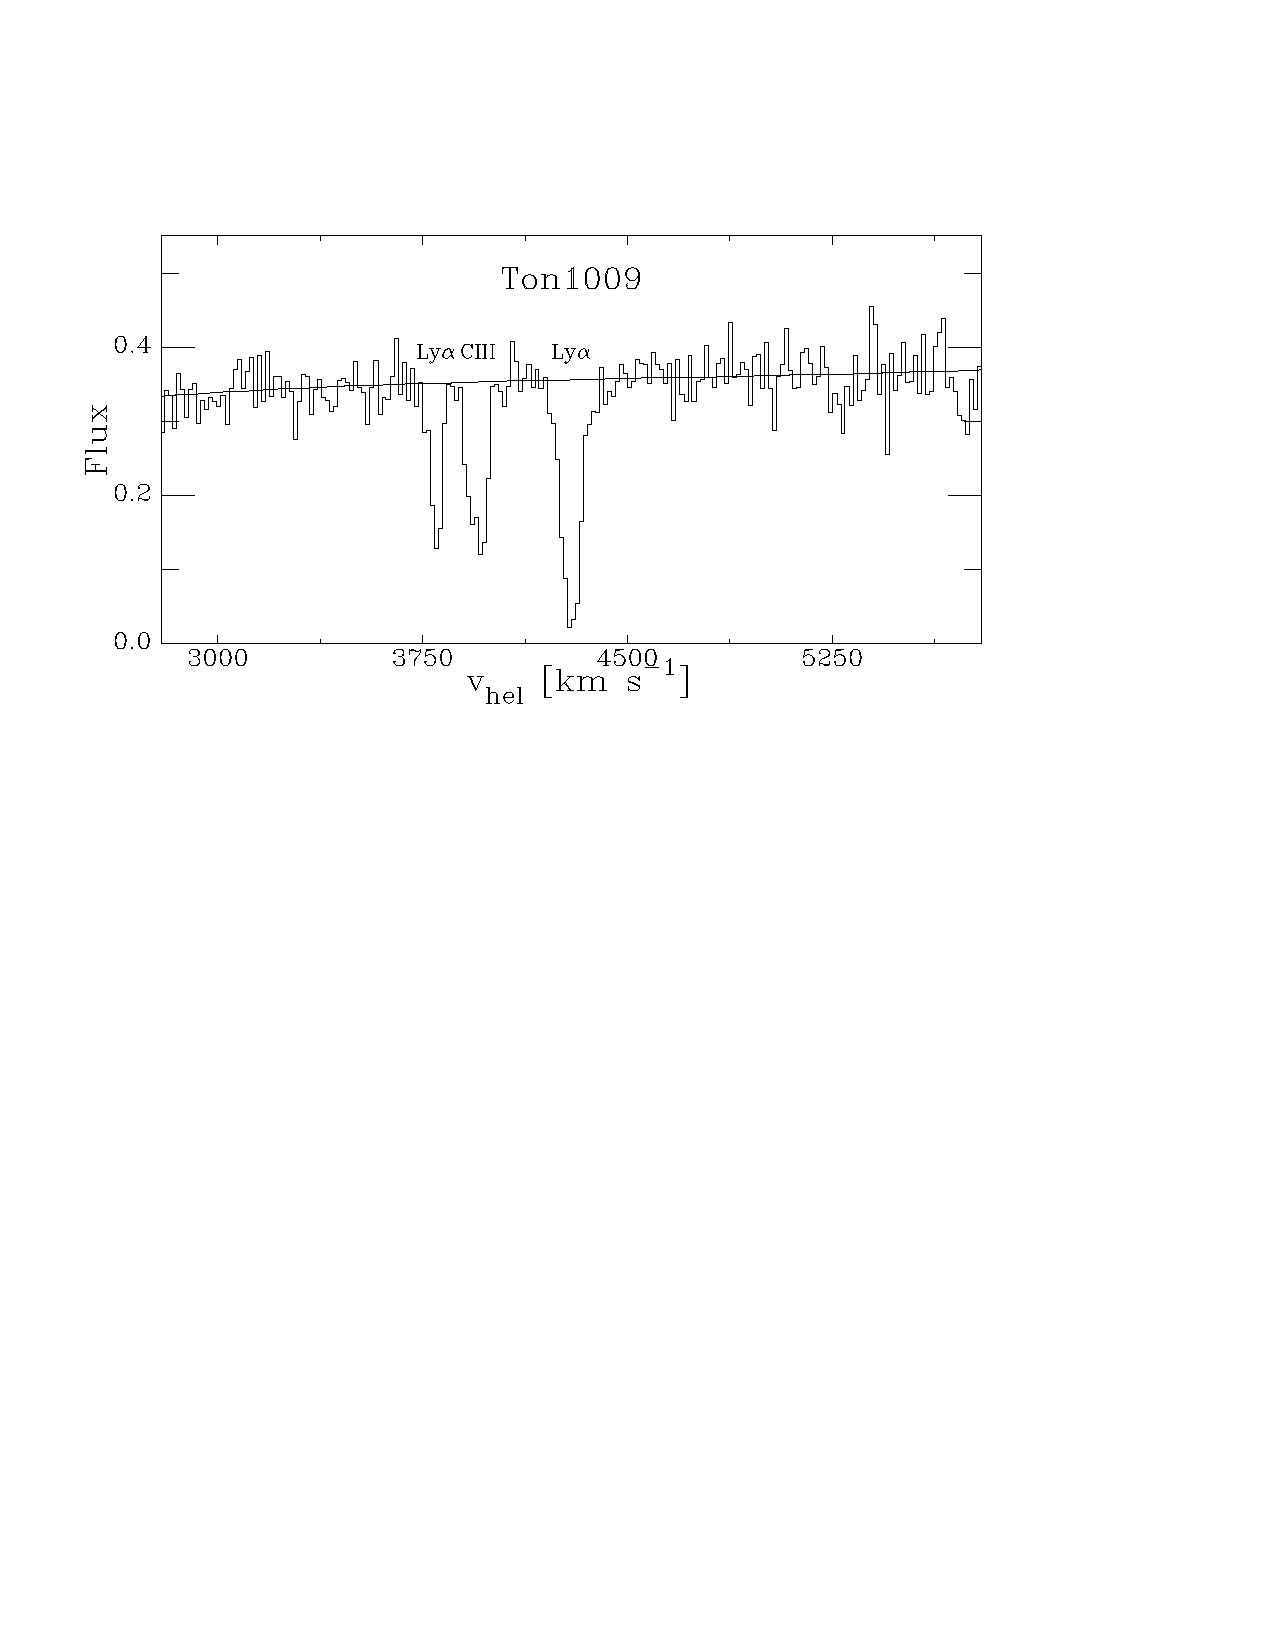
\includegraphics[width=.6\linewidth]{figTON1009_crop.pdf}}{\label{line}}
%  \subfigure[]{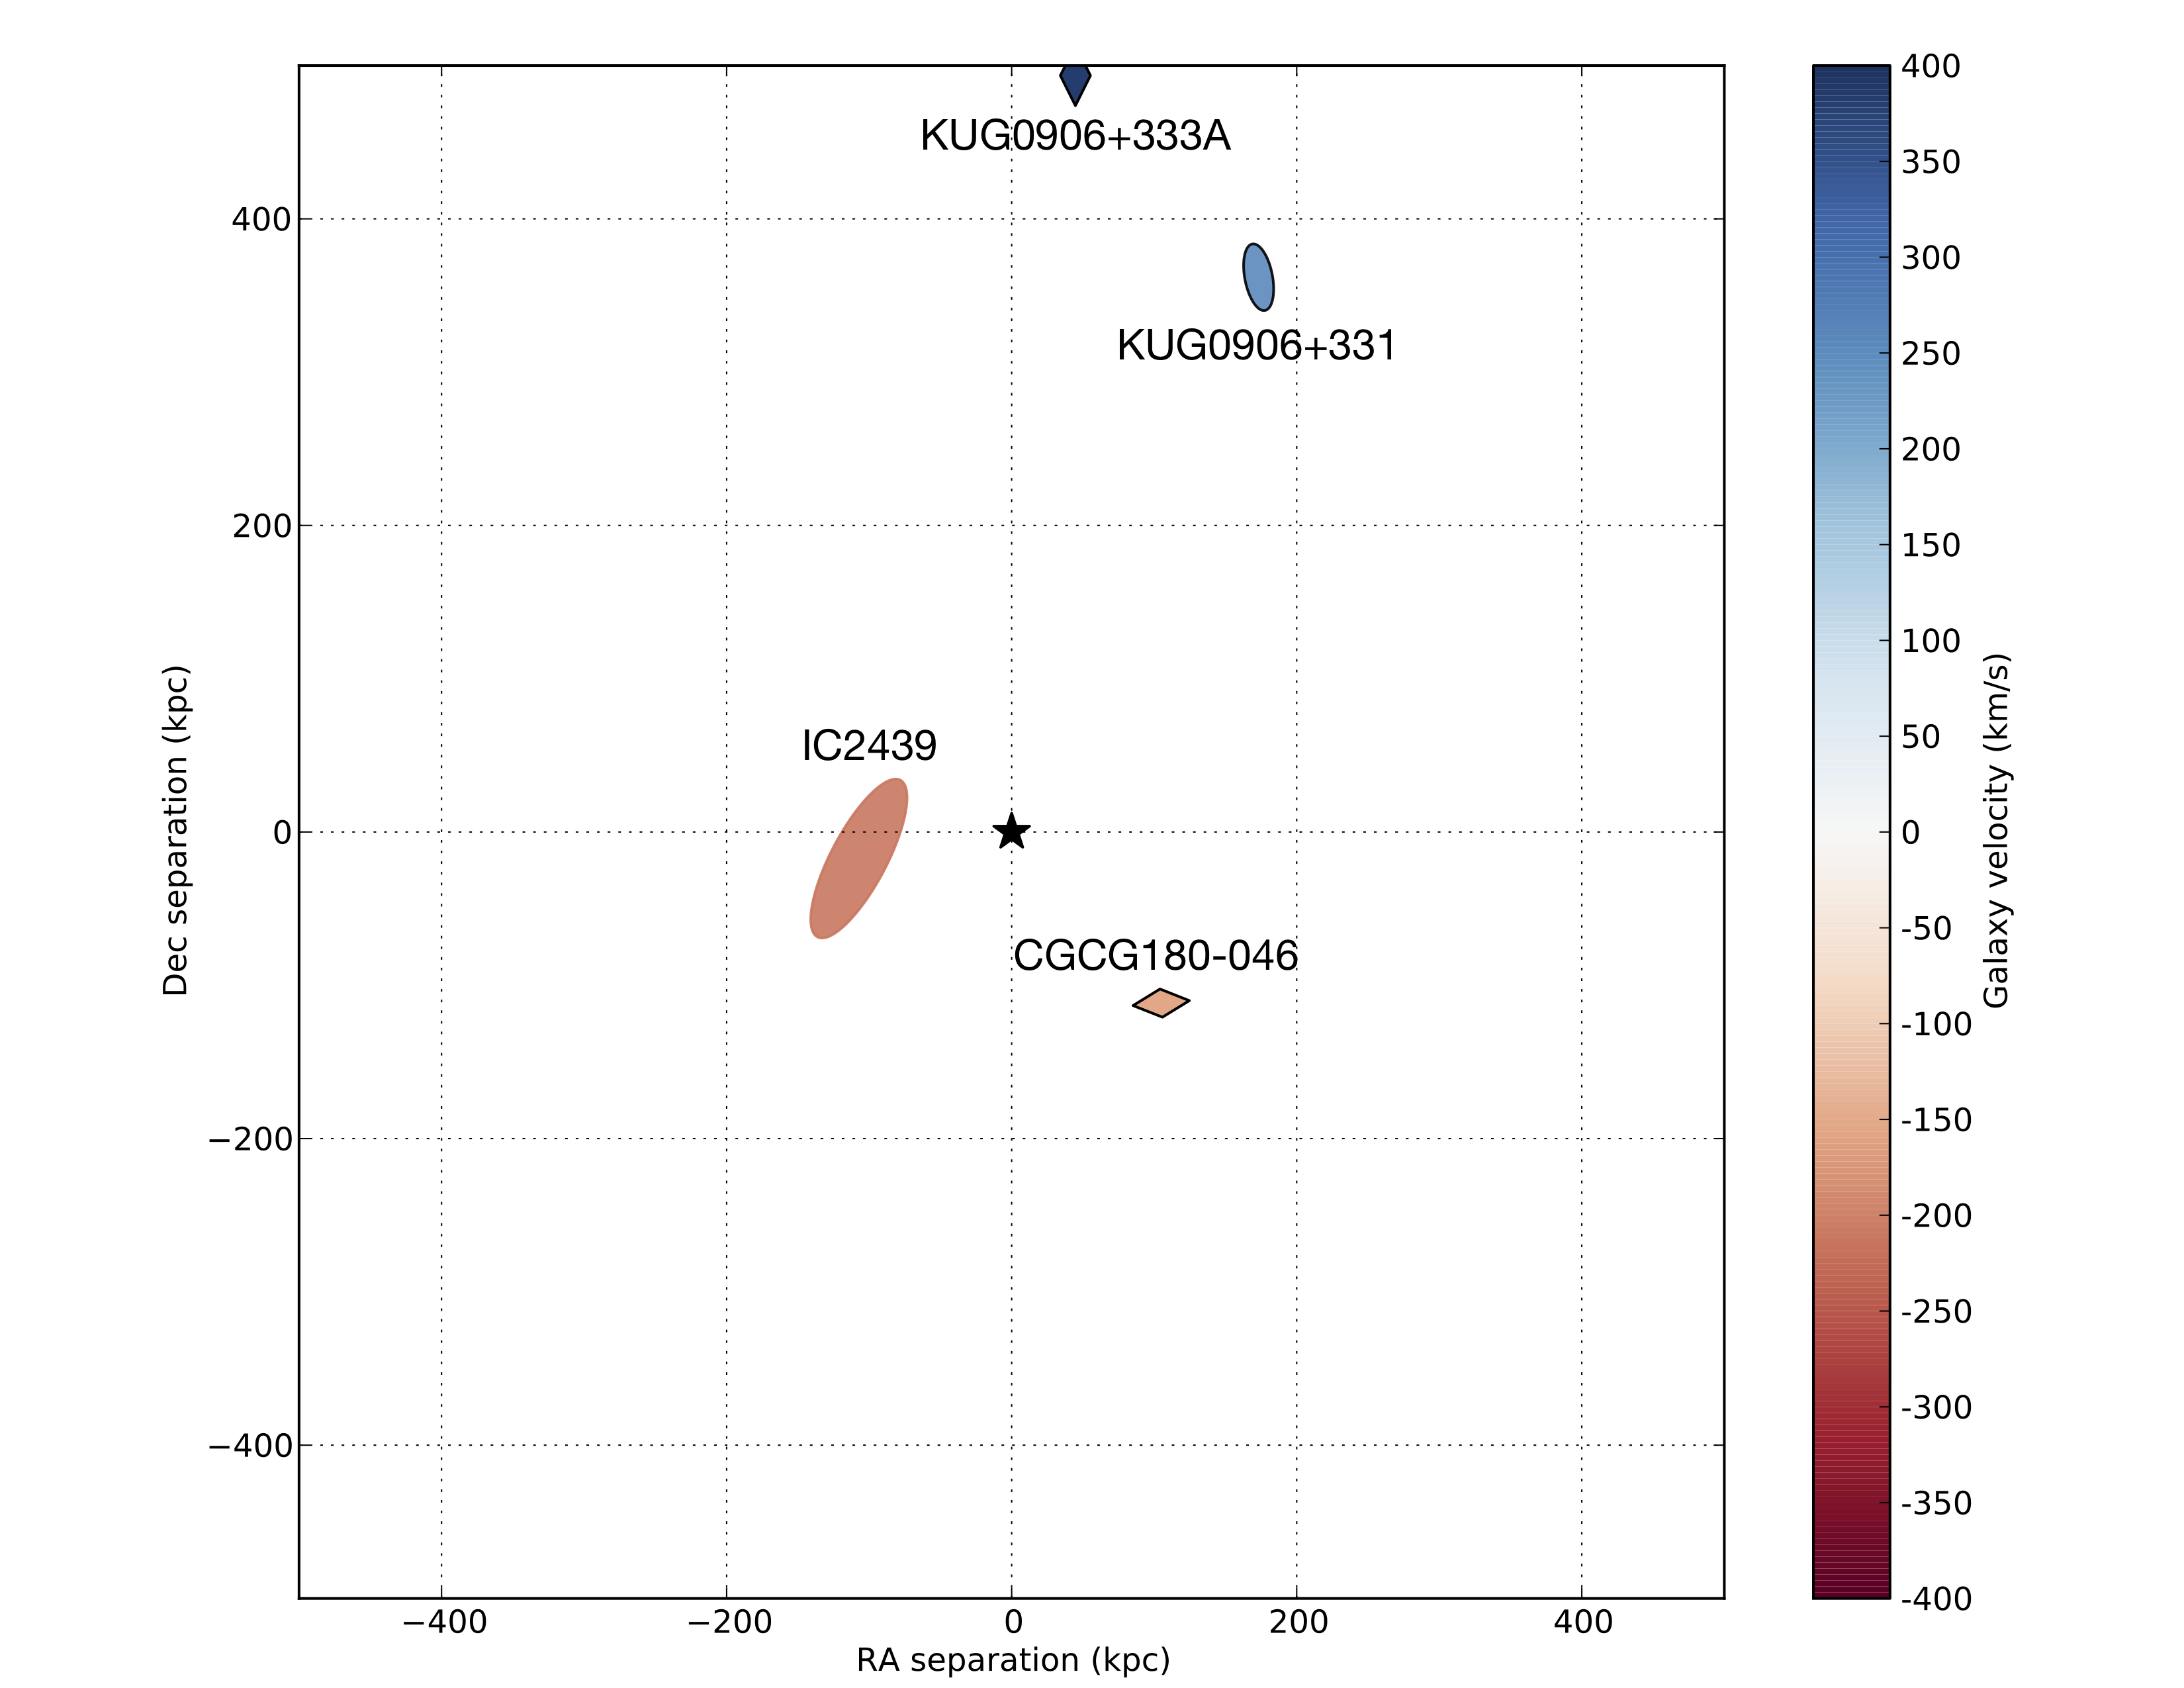
\includegraphics[width=.6\linewidth]{map_TON1009_4285_crop2_labels.png}\label{impactmap}}
%  \caption{\small{a) An example Ly$\alpha$ line found in a sightline towards target TON1009 at 4295 km/s. b) A map of \textit{all} galaxies within a 500 kpc impact parameter target TON1009 sightline and with velocity ($cz$) within 400 km/s of absorption detected at 4295 km/s (central black star). The galaxy IC2439 ($v=4494$ km/s, inclination = $71^{\circ}$) can be unambiguously paired with the Ly$\alpha$ absorption feature at $v=4295$ km/s because it is the largest and closest galaxy in both physical and velocity space to the absorption feature.}}
%\vspace{5pt}
%\end{figure}


%\noindent \textbf{\underline{3. Incompleteness}}\\

%Other studies supplement archival galaxy data with new observations, but then the search radius is usually limited to a $<10'$ field of view. For example, Mathes et al. (2014) use imaging from the WFPC2 camera on HST, but their impact parameter limit is 300 kpc, close to the commonly accepted boundary between CGM and IGM gas (based on virial radii and/or escape velocity arguments, e.g., see Stocke et al. 2013 and Mathes et al. 2014). 


%%%%%%%%%%%%%%%%%%%%%%%%%%%%%%%%%%%%%%%%%%%%%%%%%%%%%%%%%%%%%%%%%%%%%%%%%%%
%   2. ANALYSIS PLAN
%       (see Section 9.6 of the Call for Proposals)
%
%
\describearchival       % Do not delete this command.
% Enter your analysis plan here.

\noindent \textbf{\underline{1. Line Identifications and Measurements:}}

The analysis begins with aligning and combining multiple exposures to produce a single, clean spectrum. We will then apply the line identification code, the mechanics of which are relatively simple and robust. First, we manually fit gaussian profiles to all spectral features above $2\sigma$ significance. Second, this list of fits is fed into our algorithm, which produces best guess IDs for each feature. Finally, we inspect each set fits and make small adjustments as needed. In this way each spectrum is both fit by machine and checked by eye, which minimizes miss-fits and machine artifacts. This will result in a dataset of all absorption lines with ID's, velocities, equivalent widths, linewidths, and column density estimates. The time needed to ID a sightline can be as little as half an hour for an easy, low-redshift target, to several days for one at $z>1$; for the first 100 we have completed already, the median is $\sim 2$ hours.

Once ID'd, we identify and measure all spectral features in the $cz\le 10,000$ km/s redshift window. After fitting a low order (1st or 2nd) polynomial to line-free regions around each absorption line, we calculate the column density using the apparent optical depth method (see Savage $\&$ Sembach 1991), as well as by making a Voigt profile fit using the VPFIT package (see Carswell et al. 2002, Kim et al. 2007). We then derive a linewidth by calculating the second moment of the apparent optical depth profile.\\

\noindent \textbf{\underline{2. Galaxy-Absorber Matching:}}

Next, we correlate our galaxy dataset with the newly produced absorber dataset. This will produce matched absorber-galaxy systems, complete with association likelihood estimates. 

\textbf{New Nearby Galaxy Catalog:} Our nearby galaxy catalog contains over 108,000 galaxies, and is complete to $\sim0.2 L^{\**}$ at $10,000$ km/s (and progressively better towards lower redshifts). The data table contains the following entries for each galaxy: coordinates, redshift, heliocentric velocity, \textbf{CORRECTED VELOCITY}, redshift-independent-distance, inclination, position angle, morphology, extinction, photometry, group association, and alternative galaxy names. NED makes an effort to homogenize these data, but we go further by normalizing all measurements of inclination, position angle, and diameter to 2MASS $K$-band values. 2MASS values were chosen as it is an all-sky survey, and measurements are available for the majority of galaxies. Additionally, we calculate best-estimate B-band magnitudes and $L^{\**}$ values from the multitude of disparate photometry values included in NED. \\

\noindent \textbf{\underline{3. Interpretation and Publication:}}

With both the absorption line and nearby galaxy datasets in hand, we will investigate how Ly$\alpha$ equivalent width varies as a function of associated galaxy inclination, impact parameter, morphology, virial radius, azimuth angle, and system velocity with respect to absorption velocity. Particular attention will be paid to how these effects vary with proximity to the galaxies (i.e. within bins of velocity and impact parameter), so that we can understand the CGM-galaxy connection and how it evolves across a range of scales. For sightlines that lie nearby the SALT-observed galaxy disk velocity measurements, we will investigate if Ly$\alpha$ absorbers tend to co-rotate with the direction of the gaseous disk, and if so, out to what distance.

The results of these studies will be published in a series of 2 papers, published in order as ground observations become available and IDing COS spectra progresses. The first will be the study of SALT rotation curves vs Ly$\alpha$ halo absorption, the second will be the full analysis of absorber properties as functions of galaxy properties. This second paper will also include an electronic data set containing all COS IDs, absorption line measurements, and galaxy associations.


%This catalog is complete to $\sim0.2 L^{\**}$ at $10,000$ km/s (and progressively better towards lower redshifts), making it the most complete, comprehensive and up-to-date nearby galaxy catalog in existence (to be published in 2016), and is key to allowing us to draw direct comparisons between the properties of the absorbers in the CGM and the properties of galaxies on a larger scale then ever before.\\


%%%%%%%%%%%%%%%%%%%%%%%%%%%%%%%%%%%%%%%%%%%%%%%%%%%%%%%%%%%%%%%%%%%%%%%%%%%

%   3. MANAGEMENT PLAN
%       (see Section 9.7 of the Call for Proposals)
%
%  Provide a concise, but complete, management plan. This plan will be used
%  by the review panels to assess the likely scale of the proposed research
%  program. Proposers should include a schedule of the work required to
%  achieve the scientific goals of the program, a description of the roles of the
%  PI, CoIs, postdocs, and students who will perform the work, and a plan to
%  disseminate the results to the community.
%
\budgetnarrative       % Do not delete this command. CALLS the Management Plan header in the Style File (IGNORE the command name of budgetnarrative
% Enter your management plan here.

\textbf{Line Identifications and Measurements}\\
\indent Spectra prep and line IDing will be led by Wakker, with additional input by French.

\noindent \textbf{Galaxy Matching}\\
\indent Galaxy matching and final dataset preparation will be led by French.



\end{document}          % End of proposal. Do not delete this line.
                        % Everything after this command is ignored.

